% !TEX program = xelatex
\documentclass[UTF8,10pt,fontset=none]{ctexart}

\usepackage{fontspec}
\setmainfont{Times New Roman}
\setsansfont{Helvetica Neue}
\setmonofont{Menlo}
\setCJKmainfont{Songti SC}
\setCJKsansfont[BoldFont={Source Han Sans CN}]{Source Han Sans CN}
\xeCJKsetup{PunctStyle=plain}

\usepackage[
  paperwidth=176mm,
  paperheight=250mm,
  top=9mm,
  bottom=11mm,
  left=9mm,
  right=9mm,
  headheight=4mm,
  headsep=3mm,
  footskip=7mm
]{geometry}
\usepackage{amsmath,amssymb,mathtools,bm,esint}
\usepackage{enumitem}
\usepackage{booktabs,tabularx,array,longtable}
\usepackage[most]{tcolorbox}
\usepackage{tikz}
\usetikzlibrary{arrows.meta,calc}
\usepackage{pgfplots}
\pgfplotsset{compat=1.18}
\usepackage{xcolor}
\usepackage{fancyhdr}
\usepackage{titlesec}
\usepackage{needspace}
\usepackage{microtype}
\usepackage[hidelinks,unicode]{hyperref}

\definecolor{MainBlue}{HTML}{155E75}
\definecolor{DeepBlue}{HTML}{0F3D4C}
\definecolor{NoteBlue}{HTML}{EDF5F7}
\definecolor{SoftGray}{HTML}{F3F5F6}
\definecolor{RuleGray}{HTML}{B8C1C5}

\hypersetup{
  pdftitle={第17—18讲知识点原图直录},
  pdfauthor={根据所给教材图片逐项整理},
  pdfsubject={多元函数积分学预备知识与多元函数积分学},
  pdfkeywords={向量,空间解析几何,三重积分,曲线积分,曲面积分,格林公式,高斯公式,斯托克斯公式}
}

\pagestyle{fancy}
\fancyhf{}
\fancyhead[L]{\sffamily\footnotesize 第17—18讲知识点原图直录}
\fancyhead[R]{\sffamily\footnotesize B5单栏版}
\fancyfoot[C]{\sffamily\footnotesize \thepage}
\renewcommand{\headrulewidth}{0.3pt}
\renewcommand{\footrulewidth}{0pt}

\setlength{\parindent}{1em}
\setlength{\parskip}{0.22em}
\setlength{\emergencystretch}{1.5em}
\setlength{\abovedisplayskip}{3pt plus 1pt minus 1pt}
\setlength{\belowdisplayskip}{3pt plus 1pt minus 1pt}
\setlength{\abovedisplayshortskip}{2pt}
\setlength{\belowdisplayshortskip}{2pt}
\allowdisplaybreaks[3]

\ctexset{
  section={
    format=\sffamily\bfseries\Large\color{DeepBlue},
    beforeskip=7pt,
    afterskip=4pt,
    number=\chinese{section}
  },
  subsection={
    format=\sffamily\bfseries\large\color{MainBlue},
    beforeskip=5pt,
    afterskip=2pt
  },
  subsubsection={
    format=\sffamily\bfseries\normalsize\color{DeepBlue},
    beforeskip=4pt,
    afterskip=1pt
  }
}

% 方法小标题沿用紧凑的行内格式，但固定从正文版心左边界开始；
% 直接重设 paragraph，避免类文件的状态相关悬挂缩进伸入左页边。
\makeatletter
\renewcommand\paragraph{\@startsection{paragraph}{4}{\z@}%
  {3pt}{-0.75em}{\normalfont\bfseries\normalsize}}
\makeatother
% ctex 与 titlesec 组合时行内标题的标准后间距可能被吞掉；
% 将固定间隔直接计入标题盒子，确保粗体标题与后文不发生重叠。
\let\baseparagraph\paragraph
\renewcommand{\paragraph}[1]{\baseparagraph{#1\hspace{1em}}}
% 标题后紧接圈号序号时，标题单独成行并禁止在两者之间分页。
\newcommand{\paragraphline}[1]{\paragraph{#1}\leavevmode\par\nopagebreak}

\setlist[itemize]{leftmargin=1.35em,itemsep=0.12em,topsep=0.18em,parsep=0pt}
\setlist[enumerate]{leftmargin=1.55em,itemsep=0.12em,topsep=0.18em,parsep=0pt}

\newtcolorbox{notebox}[1][]{
  enhanced,breakable,
  colback=NoteBlue,colframe=MainBlue,
  boxrule=0.45pt,arc=1mm,
  left=1.2mm,right=1.2mm,top=0.8mm,bottom=0.8mm,
  before skip=2.5pt,after skip=2.5pt,
  fonttitle=\sffamily\bfseries,
  title={【注】#1}
}
\newtcolorbox{sourcebox}[1]{
  enhanced,breakable,
  colback=SoftGray,colframe=DeepBlue,
  boxrule=0.45pt,arc=1mm,
  left=1.2mm,right=1.2mm,top=0.8mm,bottom=0.8mm,
  before skip=2.5pt,after skip=2.5pt,
  fonttitle=\sffamily\bfseries,
  title={#1}
}
\newtcolorbox{theorembox}[1]{
  enhanced,breakable,
  colback=NoteBlue,colframe=DeepBlue,
  boxrule=0.65pt,arc=1mm,
  left=1.2mm,right=1.2mm,top=0.8mm,bottom=0.8mm,
  before skip=2.5pt,after skip=2.5pt,
  fonttitle=\sffamily\bfseries,
  title={#1}
}

\newcommand{\key}[1]{\textbf{\color{DeepBlue}#1}}
\newcommand{\prop}[1]{\par\noindent\textbf{性质 #1}\quad}
\newcommand{\lecturetitle}[1]{\section*{#1}}
\newcommand{\parttitle}[2]{\subsection*{#1\quad #2}}
\newcommand{\topictitle}[2]{\subsubsection*{#1\quad #2}}
\newcommand{\circnum}[1]{%
  \tikz[baseline=(char.base)]\node[
    circle,draw=DeepBlue,line width=0.45pt,
    inner sep=0.25pt,minimum size=1.45em,
    font=\sffamily\bfseries\scriptsize,text=DeepBlue
  ](char){#1};%
}
\newcommand{\circitem}[1]{\par\noindent\circnum{#1}\enspace}
\newcommand{\parenitem}[1]{\par\noindent（#1）\enspace}
\newcommand{\dd}{\mathop{}\!\mathrm d}
\newcommand{\grad}{\operatorname{grad}}
\newcommand{\diver}{\operatorname{div}}
\newcommand{\rot}{\operatorname{rot}}
\newcommand{\prj}{\operatorname{Prj}}
\newcommand{\iiintO}{\iiint\limits_{\Omega}}
\newcommand{\iintS}{\iint\limits_{\Sigma}}
\newcommand{\intL}{\int\limits_L}
\newcommand{\oiintS}{\oiint\limits_{\Sigma}}
\newcommand{\ointL}{\oint\limits_L}
\newcommand{\br}{\bm r}
\newcommand{\bF}{\bm F}
\newcommand{\bn}{\bm n}
\newcommand{\bS}{\bm S}
\newcolumntype{Y}{>{\raggedright\arraybackslash}X}

% 所有图形均由曲面方程的三维参数模型直接采样生成，不使用二维轮廓拼接。
\pgfplotsset{
  quadric model/.style={
    width=38mm,
    height=30mm,
    scale only axis,
    view={125}{24},
    axis lines=center,
    axis line style={draw=black!64,thin,-{Latex[length=1.25mm]}},
    ticks=none,
    xlabel={$x$},ylabel={$y$},zlabel={$z$},
    label style={font=\scriptsize,inner sep=0.4pt},
    enlargelimits=false,
    clip=false,
    z buffer=sort,
    axis on top=false
  },
  quadric surface/.style={
    surf,
    shader=flat,
    fill=MainBlue!28,
    draw=DeepBlue!55,
    line width=0.14pt,
    fill opacity=0.82,
    draw opacity=0.40
  },
  quadric hidden line/.style={
    draw=black!58,
    densely dashed,
    line width=0.28pt,
    opacity=0.74,
    forget plot
  }
}

% x^2/1.20^2+y^2/0.88^2+z^2=1
\newcommand{\figEllipsoid}{%
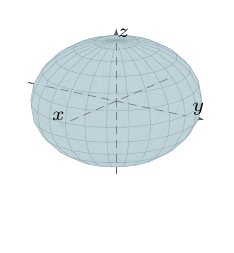
\begin{tikzpicture}[baseline=-0.5ex]
  \begin{axis}[quadric model,xmin=-1.45,xmax=1.45,ymin=-1.12,ymax=1.12,zmin=-1.20,zmax=1.20]
    \addplot3[quadric surface,samples=25,samples y=13,domain=0:360,y domain=0:180]
      ({1.20*sin(y)*cos(x)},{0.88*sin(y)*sin(x)},{cos(y)});
    \addplot3[quadric hidden line] coordinates {(-1.20,0,0) (1.20,0,0)};
    \addplot3[quadric hidden line] coordinates {(0,-0.88,0) (0,0.88,0)};
    \addplot3[quadric hidden line] coordinates {(0,0,-1) (0,0,1)};
  \end{axis}
\end{tikzpicture}}

% x^2+y^2/0.78^2-z^2=1
\newcommand{\figOneSheet}{%
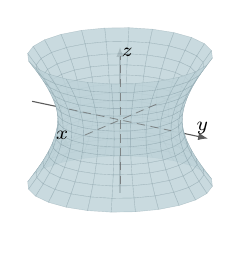
\begin{tikzpicture}[baseline=-0.5ex]
  \begin{axis}[quadric model,xmin=-1.70,xmax=1.70,ymin=-1.35,ymax=1.35,zmin=-1.25,zmax=1.25]
    \addplot3[quadric surface,samples=25,samples y=15,domain=0:360,y domain=-0.95:0.95]
      ({cosh(y)*cos(x)},{0.78*cosh(y)*sin(x)},{sinh(y)});
    \addplot3[quadric hidden line] coordinates {(-1,0,0) (1,0,0)};
    \addplot3[quadric hidden line] coordinates {(0,-0.78,0) (0,0.78,0)};
    \addplot3[quadric hidden line] coordinates {(0,0,-1.10) (0,0,1.10)};
  \end{axis}
\end{tikzpicture}}

% x^2-y^2/0.75^2-z^2/0.70^2=1，两叶分别直接建模
\newcommand{\figTwoSheet}{%
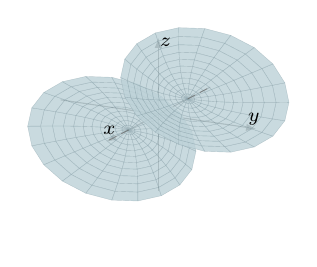
\begin{tikzpicture}[baseline=-0.5ex]
  \begin{axis}[quadric model,view={118}{22},xmin=-1.75,xmax=1.75,ymin=-1.05,ymax=1.05,zmin=-1.05,zmax=1.05]
    \addplot3[quadric surface,samples=21,samples y=12,domain=0:360,y domain=0:1.02]
      ({cosh(y)},{0.75*sinh(y)*cos(x)},{0.70*sinh(y)*sin(x)});
    \addplot3[quadric surface,samples=21,samples y=12,domain=0:360,y domain=0:1.02]
      ({-cosh(y)},{0.75*sinh(y)*cos(x)},{0.70*sinh(y)*sin(x)});
    \addplot3[quadric hidden line] coordinates {(-1.65,0,0) (-1,0,0)};
    \addplot3[quadric hidden line] coordinates {(1,0,0) (1.65,0,0)};
  \end{axis}
\end{tikzpicture}}

% x^2/1.15^2+y^2/0.88^2=z
\newcommand{\figParaboloid}{%
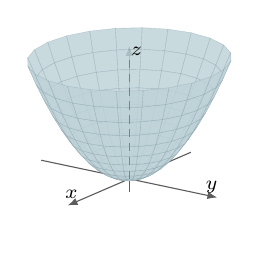
\begin{tikzpicture}[baseline=-0.5ex]
  \begin{axis}[quadric model,xmin=-1.35,xmax=1.35,ymin=-1.12,ymax=1.12,zmin=-0.15,zmax=1.55]
    \addplot3[quadric surface,samples=25,samples y=13,domain=0:360,y domain=0:1.18]
      ({1.15*y*cos(x)},{0.88*y*sin(x)},{y^2});
    \addplot3[quadric hidden line] coordinates {(0,0,0) (0,0,1.42)};
  \end{axis}
\end{tikzpicture}}

% x^2+y^2/0.78^2=z^2
\newcommand{\figCone}{%
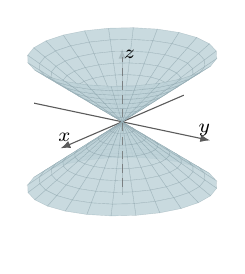
\begin{tikzpicture}[baseline=-0.5ex]
  \begin{axis}[quadric model,xmin=-1.30,xmax=1.30,ymin=-1.08,ymax=1.08,zmin=-1.35,zmax=1.35]
    \addplot3[quadric surface,samples=25,samples y=17,domain=0:360,y domain=-1.20:1.20]
      ({abs(y)*cos(x)},{0.78*abs(y)*sin(x)},{y});
    \addplot3[quadric hidden line] coordinates {(0,0,-1.20) (0,0,1.20)};
  \end{axis}
\end{tikzpicture}}

% z=0.62(y^2-x^2)
\newcommand{\figSaddle}{%
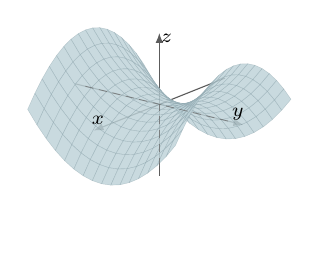
\begin{tikzpicture}[baseline=-0.5ex]
  \begin{axis}[quadric model,view={128}{25},xmin=-1.25,xmax=1.25,ymin=-1.25,ymax=1.25,zmin=-0.95,zmax=0.95]
    \addplot3[quadric surface,samples=17,samples y=17,domain=-1.10:1.10,y domain=-1.10:1.10]
      ({x},{y},{0.62*(y^2-x^2)});
    \addplot3[quadric hidden line] coordinates {(0,-1.10,0) (0,1.10,0)};
    \addplot3[quadric hidden line] coordinates {(0,0,-0.82) (0,0,0)};
  \end{axis}
\end{tikzpicture}}

% x^2+y^2/0.72^2=1，z 为自由参数
\newcommand{\figEllipticCylinder}{%
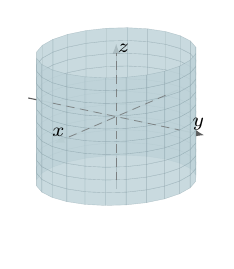
\begin{tikzpicture}[baseline=-0.5ex]
  \begin{axis}[quadric model,xmin=-1.25,xmax=1.25,ymin=-1.00,ymax=1.00,zmin=-1.20,zmax=1.20]
    \addplot3[quadric surface,samples=25,samples y=11,domain=0:360,y domain=-1.05:1.05]
      ({cos(x)},{0.72*sin(x)},{y});
    \addplot3[quadric hidden line] coordinates {(-1,0,0) (1,0,0)};
    \addplot3[quadric hidden line] coordinates {(0,-0.72,0) (0,0.72,0)};
    \addplot3[quadric hidden line] coordinates {(0,0,-1.05) (0,0,1.05)};
  \end{axis}
\end{tikzpicture}}

% x^2-y^2/0.68^2=1，z 为自由参数；两个分支分别建模
\newcommand{\figHyperbolicCylinder}{%
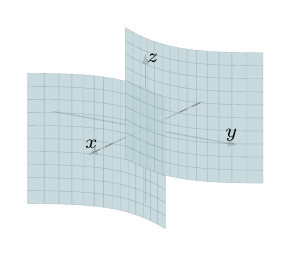
\begin{tikzpicture}[baseline=-0.5ex]
  \begin{axis}[quadric model,view={122}{23},xmin=-1.75,xmax=1.75,ymin=-1.00,ymax=1.00,zmin=-1.20,zmax=1.20]
    \addplot3[quadric surface,samples=15,samples y=11,domain=-0.95:0.95,y domain=-1.05:1.05]
      ({cosh(x)},{0.68*sinh(x)},{y});
    \addplot3[quadric surface,samples=15,samples y=11,domain=-0.95:0.95,y domain=-1.05:1.05]
      ({-cosh(x)},{0.68*sinh(x)},{y});
    \addplot3[quadric hidden line] coordinates {(-1.65,0,0) (-1,0,0)};
    \addplot3[quadric hidden line] coordinates {(1,0,0) (1.65,0,0)};
  \end{axis}
\end{tikzpicture}}

% y=0.72x^2，z 为自由参数
\newcommand{\figParabolicCylinder}{%
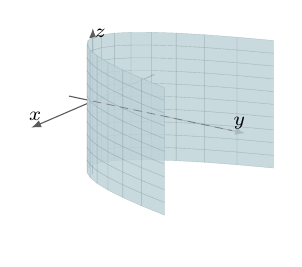
\begin{tikzpicture}[baseline=-0.5ex]
  \begin{axis}[quadric model,view={125}{24},xmin=-1.30,xmax=1.30,ymin=-0.18,ymax=1.15,zmin=-1.20,zmax=1.20]
    \addplot3[quadric surface,samples=17,samples y=11,domain=-1.15:1.15,y domain=-1.05:1.05]
      ({x},{0.72*x^2},{y});
    \addplot3[quadric hidden line] coordinates {(0,0,0) (0,1.05,0)};
  \end{axis}
\end{tikzpicture}}


\begin{document}
\fontsize{9}{11}\selectfont
\lecturetitle{第17讲\quad 多元函数积分学的预备知识（仅数学一）}

\parttitle{一}{向量代数}

\topictitle{1}{向量及其表达形式}

既有大小又有方向的量称为\key{向量}。

\begin{notebox}
两个向量，只要它们的大小相等、方向相同，它们就是相等的向量，与它们在空间中的位置无关（这也称为向量的自由性）。
\end{notebox}

向量的表达形式为 $\bm a=(a_x,a_y,a_z)=a_x\bm i+a_y\bm j+a_z\bm k$，其模为 $|\bm a|=\sqrt{a_x^2+a_y^2+a_z^2}$。

\topictitle{2}{向量的运算及其应用}

设 $\bm a=(a_x,a_y,a_z)$，$\bm b=(b_x,b_y,b_z)$，$\bm c=(c_x,c_y,c_z)$，$\bm a,\bm b,\bm c$ 均为非零向量。

\paragraphline{（1）数量积（内积、点积）及其应用}

\circitem{1} $\bm a\cdot\bm b=(a_x,a_y,a_z)\cdot(b_x,b_y,b_z)=a_xb_x+a_yb_y+a_zb_z$。

\circitem{2} $\bm a\cdot\bm b=|\bm a|\,|\bm b|\cos\theta$，则
$\displaystyle \cos\theta=\frac{\bm a\cdot\bm b}{|\bm a|\,|\bm b|}
=\frac{a_xb_x+a_yb_y+a_zb_z}
{\sqrt{a_x^2+a_y^2+a_z^2}\sqrt{b_x^2+b_y^2+b_z^2}}$，其中 $\theta$ 为 $\bm a,\bm b$ 的夹角。

\circitem{3} $\bm a\perp\bm b\Longleftrightarrow\theta=\dfrac{\pi}{2}
\Longleftrightarrow\bm a\cdot\bm b=|\bm a|\,|\bm b|\cos\theta=0
\Longleftrightarrow a_xb_x+a_yb_y+a_zb_z=0$。

\circitem{4} $\displaystyle \prj_{\bm b}\bm a
=\frac{\bm a\cdot\bm b}{|\bm b|}
=\frac{a_xb_x+a_yb_y+a_zb_z}{\sqrt{b_x^2+b_y^2+b_z^2}}
=|\bm a|\cos\theta$，称为 $\bm a$ 在 $\bm b$ 上的投影。

\paragraphline{（2）向量积（外积、叉积）及其应用}

\circitem{1}
\[
\bm a\times\bm b=
\begin{vmatrix}
\bm i&\bm j&\bm k\\
a_x&a_y&a_z\\
b_x&b_y&b_z
\end{vmatrix},
\qquad |\bm a\times\bm b|=|\bm a|\,|\bm b|\sin\theta .
\]
其中 $\bm a\times\bm b$ 的方向用右手法则确定，转向角不超过 $\pi$；$\bm a\times\bm b$ 同时垂直于 $\bm a,\bm b$，而 $|\bm a\times\bm b|$ 为以 $\bm a,\bm b$ 为邻边的平行四边形面积。

\circitem{2} $\bm a\parallel\bm b\Longleftrightarrow\theta=0$ 或 $\pi
\Longleftrightarrow\bm a\times\bm b=\bm0
\Longleftrightarrow\dfrac{a_x}{b_x}=\dfrac{a_y}{b_y}=\dfrac{a_z}{b_z}$。

\paragraphline{（3）混合积及其应用}

\circitem{1}
\[
[\bm a,\bm b,\bm c]=(\bm a\times\bm b)\cdot\bm c
=\begin{vmatrix}
a_x&a_y&a_z\\
b_x&b_y&b_z\\
c_x&c_y&c_z
\end{vmatrix}.
\]

\circitem{2} $[\bm a,\bm b,\bm c]=0\Longleftrightarrow\bm a,\bm b,\bm c$ 共面；$|[\bm a,\bm b,\bm c]|$ 是以 $\bm a,\bm b,\bm c$ 为棱的平行六面体体积。

\topictitle{3}{向量的方向角和方向余弦}

\parenitem{1} 非零向量 $\bm a$ 与 $x$ 轴、$y$ 轴和 $z$ 轴正向的夹角 $\alpha,\beta,\gamma$，称为 $\bm a$ 的方向角。

\parenitem{2} $\cos\alpha,\cos\beta,\cos\gamma$ 称为 $\bm a$ 的方向余弦，且
$\displaystyle \cos\alpha=\frac{a_x}{|\bm a|}$，
$\displaystyle \cos\beta=\frac{a_y}{|\bm a|}$，
$\displaystyle \cos\gamma=\frac{a_z}{|\bm a|}$。

\parenitem{3} $\displaystyle \bm a^\circ=\frac{\bm a}{|\bm a|}
=(\cos\alpha,\cos\beta,\cos\gamma)$ 称为向量 $\bm a$ 的单位向量。

\parenitem{4} 任意向量
\[
\bm r=x\bm i+y\bm j+z\bm k
=r(\cos\alpha,\cos\beta,\cos\gamma),
\qquad r=\sqrt{x^2+y^2+z^2},
\]
称为位置向量（表示方向的向量），其中
$\displaystyle \cos\alpha=\frac{x}{r}$，
$\displaystyle \cos\beta=\frac{y}{r}$，
$\displaystyle \cos\gamma=\frac{z}{r}$，且
$\cos^2\alpha+\cos^2\beta+\cos^2\gamma=1$。

\parttitle{二}{空间平面与直线}

\topictitle{1}{平面方程}

以下假设平面的法向量为 $\bm n=(A,B,C)$。

\circitem{1} 一般式：$Ax+By+Cz+D=0$。

\circitem{2} 点法式：$A(x-x_0)+B(y-y_0)+C(z-z_0)=0$。

\circitem{3} 三点式：
\[
\begin{vmatrix}
x-x_1&y-y_1&z-z_1\\
x-x_2&y-y_2&z-z_2\\
x-x_3&y-y_3&z-z_3
\end{vmatrix}=0,
\]
其中平面过不共线的三点 $P_i(x_i,y_i,z_i)$（$i=1,2,3$）。

\circitem{4} 截距式：$\displaystyle \frac{x}{a}+\frac{y}{b}+\frac{z}{c}=1$，平面过 $(a,0,0),(0,b,0),(0,0,c)$ 三点。

\circitem{5} 平面束方程：设
$\pi_i:A_ix+B_iy+C_iz+D_i=0$（$i=1,2$），且
$A_1,B_1,C_1$ 与 $A_2,B_2,C_2$ 不成比例，则过两平面交线
\[
L:\begin{cases}
A_1x+B_1y+C_1z+D_1=0,\\
A_2x+B_2y+C_2z+D_2=0
\end{cases}
\]
的平面束方程为
$A_1x+B_1y+C_1z+D_1+\lambda(A_2x+B_2y+C_2z+D_2)=0$（不含 $\pi_2$），或
$A_2x+B_2y+C_2z+D_2+\lambda(A_1x+B_1y+C_1z+D_1)=0$（不含 $\pi_1$）。

\topictitle{2}{直线方程}

以下假设直线的方向向量 $\bm\tau=(l,m,n)$。

\circitem{1} 一般式：
\[
\begin{cases}
A_1x+B_1y+C_1z+D_1=0,\\
A_2x+B_2y+C_2z+D_2=0,
\end{cases}
\qquad
\bm n_1=(A_1,B_1,C_1),\quad
\bm n_2=(A_2,B_2,C_2),
\]
其中 $\bm n_1$ 不平行于 $\bm n_2$。

\begin{notebox}
其几何背景是两个平面的交线，且该直线的方向向量 $\bm\tau=\bm n_1\times\bm n_2$。
\end{notebox}

\circitem{2} 点向式：$\displaystyle
\frac{x-x_0}{l}=\frac{y-y_0}{m}=\frac{z-z_0}{n}$。

\circitem{3} 参数式：$x=x_0+lt,\ y=y_0+mt,\ z=z_0+nt$，$P_0(x_0,y_0,z_0)$ 为直线上的已知点，$t$ 为参数。

\circitem{4} 两点式：
\[
\frac{x-x_1}{x_2-x_1}
=\frac{y-y_1}{y_2-y_1}
=\frac{z-z_1}{z_2-z_1},
\]
直线过不同的两点 $P_i(x_i,y_i,z_i)$（$i=1,2$）。

\topictitle{3}{位置关系}

\paragraph{（1）点到直线的距离}

点 $M_1(x_1,y_1,z_1)$ 到直线
$\displaystyle L:\frac{x-x_0}{l}=\frac{y-y_0}{m}=\frac{z-z_0}{n}$
的距离为
$\displaystyle d=\frac{|\bm\tau\times\overrightarrow{M_1M_0}|}{|\bm\tau|}$，
其中 $\overrightarrow{M_1M_0}=(x_0-x_1,y_0-y_1,z_0-z_1)$，$M_0=(x_0,y_0,z_0)$，$\bm\tau=(l,m,n)$。

\begin{notebox}
在二维平面上，直线 $L$ 的方程为 $Ax+By+C=0$，点 $P_0$ 的坐标为 $(x_0,y_0)$，则
$\displaystyle d=\frac{|Ax_0+By_0+C|}{\sqrt{A^2+B^2}}$。
\end{notebox}

\paragraph{（2）点到平面的距离}

点 $P_0(x_0,y_0,z_0)$ 到平面 $Ax+By+Cz+D=0$ 的距离为
$\displaystyle d=\frac{|Ax_0+By_0+Cz_0+D|}{\sqrt{A^2+B^2+C^2}}$。

\paragraph{（3）直线与直线}

设 $\bm\tau_1=(l_1,m_1,n_1)$，$\bm\tau_2=(l_2,m_2,n_2)$ 分别为直线 $L_1,L_2$ 的方向向量。

\circitem{1} $L_1\perp L_2\Longleftrightarrow\bm\tau_1\perp\bm\tau_2
\Longleftrightarrow l_1l_2+m_1m_2+n_1n_2=0$。

\circitem{2} $L_1\parallel L_2\Longleftrightarrow\bm\tau_1\parallel\bm\tau_2
\Longleftrightarrow\dfrac{l_1}{l_2}=\dfrac{m_1}{m_2}=\dfrac{n_1}{n_2}$。

\circitem{3} 直线 $L_1,L_2$ 的夹角
$\displaystyle \theta=\arccos\frac{|\bm\tau_1\cdot\bm\tau_2|}
{|\bm\tau_1|\,|\bm\tau_2|}$，其中
$\theta=\min\{(\bm\tau_1,\bm\tau_2),\pi-(\bm\tau_1,\bm\tau_2)\}
\in[0,\frac{\pi}{2}]$。

\paragraph{（4）平面与平面}

设平面 $\pi_1,\pi_2$ 的法向量分别为 $\bm n_1=(A_1,B_1,C_1)$，$\bm n_2=(A_2,B_2,C_2)$。

\circitem{1} $\pi_1\perp\pi_2\Longleftrightarrow\bm n_1\perp\bm n_2
\Longleftrightarrow A_1A_2+B_1B_2+C_1C_2=0$。

\circitem{2} $\pi_1\parallel\pi_2\Longleftrightarrow\bm n_1\parallel\bm n_2
\Longleftrightarrow\dfrac{A_1}{A_2}=\dfrac{B_1}{B_2}=\dfrac{C_1}{C_2}$。

\circitem{3} 平面 $\pi_1,\pi_2$ 的夹角
$\displaystyle \theta=\arccos\frac{|\bm n_1\cdot\bm n_2|}
{|\bm n_1|\,|\bm n_2|}$，其中
$\theta=\min\{(\bm n_1,\bm n_2),\pi-(\bm n_1,\bm n_2)\}
\in[0,\frac{\pi}{2}]$。

\paragraph{（5）平面与直线}

设直线 $L$ 的方向向量为 $\bm\tau=(l,m,n)$，平面 $\pi$ 的法向量为 $\bm n=(A,B,C)$。

\circitem{1} $L\perp\pi\Longleftrightarrow\bm\tau\parallel\bm n
\Longleftrightarrow\dfrac{l}{A}=\dfrac{m}{B}=\dfrac{n}{C}$。

\circitem{2} $L\parallel\pi\Longleftrightarrow\bm\tau\perp\bm n
\Longleftrightarrow Al+Bm+Cn=0$。

\circitem{3} 直线 $L$ 与平面 $\pi$ 的夹角
$\displaystyle \theta=\arcsin\frac{|\bm\tau\cdot\bm n|}
{|\bm\tau|\,|\bm n|}$，其中
$\theta=\left|\frac{\pi}{2}-(\bm\tau,\bm n)\right|
\in[0,\frac{\pi}{2}]$。

\parttitle{三}{空间曲线与曲面}

\topictitle{1}{空间曲线}

\parenitem{1} 一般式：
$\displaystyle \Gamma:\begin{cases}F(x,y,z)=0,\\G(x,y,z)=0.\end{cases}$

\begin{notebox}
其几何背景为两个曲面的交线。
\end{notebox}

\parenitem{2} 参数方程：
$\displaystyle \Gamma:\begin{cases}
x=\varphi(t),\\y=\psi(t),\\z=\omega(t),
\end{cases}\ t\in[\alpha,\beta]$。

\begin{notebox}
在方程组 $\begin{cases}F(x,y,z)=0,\\G(x,y,z)=0\end{cases}$ 中选取某直角坐标变量为自变量（看作参数），解出其他两个变量为此变量的函数，即得参数式；若不便解出，可另用新变量作参数。
\end{notebox}

\parenitem{3} 在坐标面上的投影。

以求曲线 $\Gamma$ 在 $xOy$ 平面上的投影曲线为例：将
$\displaystyle \Gamma:\begin{cases}F(x,y,z)=0,\\G(x,y,z)=0\end{cases}$
中的 $z$ 消去，得到 $\varphi(x,y)=0$，则曲线 $\Gamma$ 在 $xOy$ 面上的投影曲线包含于
$\displaystyle \begin{cases}\varphi(x,y)=0,\\z=0.\end{cases}$
曲线在其他平面上的投影曲线可类似求得。

\begin{notebox}
若空间曲线由方程组 $\begin{cases}F(x,y,z)=0,\\G(x,y,z)=0\end{cases}$ 给出，则消去某变量（例如消去 $z$），可得该曲线在 $z=0$ 平面上的投影曲线方程
$\begin{cases}f(x,y)=0,\\z=0.\end{cases}$
如果 $f(x,y)=0$ 能容易地写成参数式 $x=x(t),y=y(t)$，代入原曲线方程中，若能解得单值的 $z=z(t)$，则原曲线的参数式为 $x=x(t),y=y(t),z=z(t)$。
\end{notebox}

\topictitle{2}{空间曲面}

\parenitem{1} 曲面方程：$F(x,y,z)=0$。

\parenitem{2} 二次曲面。

\begingroup
\renewcommand{\arraystretch}{1.13}
\setlength{\LTpre}{2pt}
\setlength{\LTpost}{3pt}
\begin{longtable}{@{}p{27mm}p{75mm}>{\centering\arraybackslash}p{45mm}@{}}
\toprule
\textbf{曲面名称} & \textbf{方程与截痕注释} & \textbf{图形} \\
\midrule
\endfirsthead
\toprule
\textbf{曲面名称} & \textbf{方程与截痕注释} & \textbf{图形（续）} \\
\midrule
\endhead
\bottomrule
\endfoot

\key{椭球面} &
$\displaystyle\frac{x^2}{a^2}+\frac{y^2}{b^2}+\frac{z^2}{c^2}=1$。
$a=b=c$ 时为球面；用平行于坐标面的平面截取，截痕为椭圆或圆。 &
\figEllipsoid \\[1mm]\midrule

\key{单叶双曲面} &
$\displaystyle\frac{x^2}{a^2}+\frac{y^2}{b^2}-\frac{z^2}{c^2}=1$（两正一负）。
用 $x=k_1$ 或 $y=k_2$ 截得双曲线；用 $z=k_3$ 截得椭圆或圆。 &
\figOneSheet \\[1mm]\midrule

\key{双叶双曲面} &
$\displaystyle\frac{x^2}{a^2}-\frac{y^2}{b^2}-\frac{z^2}{c^2}=1$（一正两负，正号对应中心轴）。
用 $y=k$ 或 $z=k$ 截得双曲线；用 $x=k$（$|k|>|a|$）截得椭圆或圆。 &
\figTwoSheet \\[1mm]\midrule

\key{椭圆抛物面} &
$\displaystyle\frac{x^2}{2p}+\frac{y^2}{2q}=z\ (p,q>0)$。
一般考 $p=q$；用 $x=k$ 或 $y=k$ 截得抛物线，用 $z=k$（$k>0$）截得椭圆或圆。 &
\figParaboloid \\[1mm]\midrule

\key{椭圆锥面} &
$\displaystyle\frac{x^2}{a^2}+\frac{y^2}{b^2}=\frac{z^2}{c^2}$。
一般考 $a=b$；$z=\sqrt{x^2+y^2}$ 只有上半部分。 &
\figCone \\[1mm]\midrule

\key{双曲抛物面（马鞍面）} &
$\displaystyle-\frac{x^2}{2p}+\frac{y^2}{2q}=z\ (p,q>0)$。
用 $z=k$ 截得双曲线，用 $x=k$ 或 $y=k$ 截得抛物线。常见形式 $z=xy$；令 $u=y+x,v=y-x$，则 $z=uv$。 &
\figSaddle
\end{longtable}
\endgroup

\parenitem{3} 柱面：动直线沿定曲线平行移动所形成的曲面。

\begingroup
\renewcommand{\arraystretch}{1.13}
\setlength{\LTpre}{2pt}
\setlength{\LTpost}{3pt}
\begin{longtable}{@{}p{27mm}p{75mm}>{\centering\arraybackslash}p{45mm}@{}}
\toprule
\textbf{曲面名称} & \textbf{方程与注释} & \textbf{图形} \\
\midrule
\endfirsthead
\toprule
\textbf{曲面名称} & \textbf{方程与注释} & \textbf{图形（续）} \\
\midrule
\endhead
\bottomrule
\endfoot

\key{椭圆柱面} &
$\displaystyle\frac{x^2}{a^2}+\frac{y^2}{b^2}=1$。
准线为椭圆或圆；方程缺少 $z$，母线平行于 $z$ 轴。 &
\figEllipticCylinder \\[1mm]\midrule

\key{双曲柱面} &
$\displaystyle\frac{x^2}{a^2}-\frac{y^2}{b^2}=1$。
准线为双曲线；方程缺少 $z$，母线平行于 $z$ 轴。 &
\figHyperbolicCylinder \\[1mm]\midrule

\key{抛物柱面} &
$\displaystyle y=ax^2\ (a>0)$。
准线为抛物线；方程缺少 $z$，母线平行于 $z$ 轴。 &
\figParabolicCylinder
\end{longtable}
\endgroup

\parenitem{4} 旋转曲面：曲线 $\Gamma$ 绕一条定直线旋转一周所形成的曲面。

设旋转轴经过点 $M_0(x_0,y_0,z_0)$，方向向量为 $\bm\tau=(l,m,n)$；母线上任取一点 $M_1(x_1,y_1,z_1)$，过 $M_1$ 的纬圆上的任意一点为 $P(x,y,z)$，则
\[
\begin{cases}
l(x-x_1)+m(y-y_1)+n(z-z_1)=0,\\
(x-x_0)^2+(y-y_0)^2+(z-z_0)^2
=(x_1-x_0)^2+(y_1-y_0)^2+(z_1-z_0)^2.
\end{cases}
\]
与方程 $F(x_1,y_1,z_1)=0$ 和 $G(x_1,y_1,z_1)=0$ 联立，消去 $x_1,y_1,z_1$，便可得到旋转曲面的方程。

\begin{notebox}
常考曲线
$\displaystyle \Gamma:\begin{cases}F(x,y,z)=0,\\G(x,y,z)=0\end{cases}$
绕 $z$ 轴旋转一周而成的旋转曲面。取 $M_1(x_1,y_1,z_1)$，则
$x^2+y^2=x_1^2+y_1^2$ 且 $z=z_1$；从
$\begin{cases}F(x_1,y_1,z)=0,\\G(x_1,y_1,z)=0,\\x^2+y^2=x_1^2+y_1^2\end{cases}$
中消去 $x_1,y_1$ 即得。若能解出 $x_1=f_1(z),y_1=f_2(z)$，则
$x^2+y^2=[f_1(z)]^2+[f_2(z)]^2$。
\end{notebox}

\parttitle{四}{多元函数微分学的几何应用}

\topictitle{1}{空间曲线的切线与法平面}

\parenitem{1} 用参数方程给出曲线：
$x=x(t),y=y(t),z=z(t)$，$t\in I$。若在 $t=t_0$ 时三个导数不同时为 $0$，则曲线在 $P_0(x_0,y_0,z_0)$ 处的切向量
$\bm\tau=(x'(t_0),y'(t_0),z'(t_0))$；切线方程
$\displaystyle \frac{x-x_0}{x'(t_0)}
=\frac{y-y_0}{y'(t_0)}
=\frac{z-z_0}{z'(t_0)}$；法平面方程
$x'(t_0)(x-x_0)+y'(t_0)(y-y_0)+z'(t_0)(z-z_0)=0$。

\parenitem{2} 用方程组给出曲线：
$\displaystyle \begin{cases}F(x,y,z)=0,\\G(x,y,z)=0.\end{cases}$
曲线在 $P_0$ 处的切向量为
\[
\bm\tau=
\begin{vmatrix}
\bm i&\bm j&\bm k\\
F_x&F_y&F_z\\
G_x&G_y&G_z
\end{vmatrix}_{P_0}
=\nabla F(P_0)\times\nabla G(P_0).
\]
若记 $\bm\tau=(A,B,C)$，则切线方程为
$\displaystyle \frac{x-x_0}{A}=\frac{y-y_0}{B}=\frac{z-z_0}{C}$，
法平面方程为 $A(x-x_0)+B(y-y_0)+C(z-z_0)=0$。

\topictitle{2}{空间曲面的切平面与法线}

\parenitem{1} 用隐式方程给出曲面：$F(x,y,z)=0$，其中 $F$ 的一阶偏导数连续。曲面在 $P_0(x_0,y_0,z_0)$ 处的法向量
$\bm n=(F_x(P_0),F_y(P_0),F_z(P_0))$；切平面方程
$F_x(P_0)(x-x_0)+F_y(P_0)(y-y_0)+F_z(P_0)(z-z_0)=0$；法线方程
$\displaystyle \frac{x-x_0}{F_x(P_0)}
=\frac{y-y_0}{F_y(P_0)}
=\frac{z-z_0}{F_z(P_0)}$。

\parenitem{2} 用显式函数给出曲面：$z=f(x,y)$，其中 $f$ 的一阶偏导数连续。曲面在 $P_0(x_0,y_0,z_0)$ 处取方向向下的法向量
$\bm n=(f_x(x_0,y_0),f_y(x_0,y_0),-1)$；切平面方程
$f_x(x_0,y_0)(x-x_0)+f_y(x_0,y_0)(y-y_0)-(z-z_0)=0$；法线方程
$\displaystyle \frac{x-x_0}{f_x(x_0,y_0)}
=\frac{y-y_0}{f_y(x_0,y_0)}
=\frac{z-z_0}{-1}$。

\begin{notebox}
若曲面上任一点的法向量都与某一固定向量 $\bm\tau$ 垂直，即 $\nabla F(x,y,z)\cdot\bm\tau=0$ 恒成立，则该曲面是以 $\bm\tau$ 为母线方向的柱面。
\end{notebox}

\parttitle{五}{场论初步}

\topictitle{1}{方向导数}

\key{定义}\quad 设三元函数 $u=u(x,y,z)$ 在点 $P_0(x_0,y_0,z_0)$ 的某空间邻域 $U\subset\mathbb R^3$ 内有定义，$l$ 为从点 $P_0$ 出发的射线，$P(x,y,z)$ 为 $l$ 上且在 $U$ 内的任一点，令
$x-x_0=t\cos\alpha$，$y-y_0=t\cos\beta$，$z-z_0=t\cos\gamma$。若极限
\[
\lim_{t\to0^+}\frac{u(P)-u(P_0)}{t}
=\lim_{t\to0^+}
\frac{u(x_0+t\cos\alpha,y_0+t\cos\beta,z_0+t\cos\gamma)-u(x_0,y_0,z_0)}{t}
\]
存在，则称此极限为函数 $u=u(x,y,z)$ 在点 $P_0$ 沿方向 $l$ 的方向导数，记作
$\left.\dfrac{\partial u}{\partial l}\right|_{P_0}$。

\begin{theorembox}{定理（方向导数的计算公式）}
设三元函数 $u=u(x,y,z)$ 在点 $P_0(x_0,y_0,z_0)$ 处可微分，则 $u$ 在点 $P_0$ 沿任一方向 $l$ 的方向导数都存在，且
\[
\left.\frac{\partial u}{\partial l}\right|_{P_0}
=u_x(P_0)\cos\alpha+u_y(P_0)\cos\beta+u_z(P_0)\cos\gamma,
\]
其中 $\cos\alpha,\cos\beta,\cos\gamma$ 为方向 $l$ 的方向余弦。
\end{theorembox}

\begin{notebox}
二元函数 $f(x,y)$ 的情况与三元函数类似。
\end{notebox}

\topictitle{2}{梯度}

\key{定义}\quad 设三元函数 $u=u(x,y,z)$ 在点 $P_0(x_0,y_0,z_0)$ 处具有一阶连续偏导数，则定义梯度为

\noindent$\left.\grad u\right|_{P_0}=(u_x(P_0),u_y(P_0),u_z(P_0))$。

\begin{notebox}
$\grad(u\pm v)=\grad u\pm\grad v$；
$\grad(uv)=v\grad u+u\grad v$；
$\displaystyle \grad\!\left(\frac uv\right)
=\frac{v\grad u-u\grad v}{v^2}$（$v\ne0$）。
\end{notebox}

\topictitle{3}{方向导数与梯度的关系}

由方向导数的计算公式与梯度的定义，可得
$\displaystyle \left.\frac{\partial u}{\partial l}\right|_{P_0}
=\left.\grad u\right|_{P_0}\cdot\bm l^\circ
=\left|\left.\grad u\right|_{P_0}\right|\cos\theta$，
其中 $\theta$ 为 $\left.\grad u\right|_{P_0}$ 与 $\bm l^\circ$ 的夹角。

\circitem{1} 当 $\cos\theta=1$ 时，$\left.\dfrac{\partial u}{\partial l}\right|_{P_0}$ 有最大值。

\circitem{2} 当 $\cos\theta=0$，即 $\theta=\dfrac{\pi}{2}$ 时，向量 $l$ 与梯度垂直，有
$\left.\dfrac{\partial u}{\partial l}\right|_{P_0}=0$，即变化率为 $0$。

于是有重要结论：函数在某点的梯度是一个向量，它的方向与取得最大方向导数的方向一致，而它的模为方向导数的最大值：
$\displaystyle |\grad u|=\sqrt{u_x^2+u_y^2+u_z^2}$。

\topictitle{4}{散度}

\key{定义}\quad 设向量场
$\bm A(x,y,z)=P(x,y,z)\bm i+Q(x,y,z)\bm j+R(x,y,z)\bm k$，则
$\displaystyle \diver\bm A=\frac{\partial P}{\partial x}
+\frac{\partial Q}{\partial y}
+\frac{\partial R}{\partial z}$，叫作向量场 $\bm A$ 的散度。

\topictitle{5}{旋度}

\key{定义}\quad 设向量场
$\bm A(x,y,z)=P(x,y,z)\bm i+Q(x,y,z)\bm j+R(x,y,z)\bm k$，则
\[
\rot\bm A=
\begin{vmatrix}
\bm i&\bm j&\bm k\\
\dfrac{\partial}{\partial x}&\dfrac{\partial}{\partial y}&\dfrac{\partial}{\partial z}\\
P&Q&R
\end{vmatrix},
\]
叫作向量场 $\bm A$ 的旋度。

\begin{notebox}
设 $z=f(x,y)$ 可微，记不共线的方向
$\bm l_1^\circ=(\cos\alpha_1,\cos\beta_1)$ 与
$\bm l_2^\circ=(\cos\alpha_2,\cos\beta_2)$，且
$\begin{vmatrix}\cos\alpha_1&\cos\beta_1\\
\cos\alpha_2&\cos\beta_2\end{vmatrix}\ne0$。

（1）若沿两个方向的方向导数不全为 $0$，则相应非齐次方程组有唯一解。

（2）若沿两个方向的方向导数均为 $0$，则 $f_x=f_y=0$，故 $\dd f=0$，从而 $f(x,y)$ 为常数。
\end{notebox}

\clearpage
\lecturetitle{第18讲\quad 多元函数积分学（仅数学一）}

\parttitle{一}{三重积分}

\topictitle{1}{概念}

设 $f(x,y,z)$ 是空间有界闭区域 $\Omega$ 上的有界函数，将 $\Omega$ 任意分成 $n$ 个小闭区域
\[
\Delta v_1,\Delta v_2,\ldots,\Delta v_n,
\]
其中 $\Delta v_i$ 表示第 $i$ 个小闭区域，也表示它的体积。在每个 $\Delta v_i$ 上任取一点
$(\xi_i,\eta_i,\zeta_i)$，作乘积 $f(\xi_i,\eta_i,\zeta_i)\Delta v_i$，并作和
\[
\sum_{i=1}^{n}f(\xi_i,\eta_i,\zeta_i)\Delta v_i.
\]
如果当各小闭区域直径中的最大值 $\lambda$ 趋于零时，这个和的极限总存在，并且与 $\Delta v_i$ 的分法及 $(\xi_i,\eta_i,\zeta_i)$ 的取法均无关，则称此极限为函数 $f(x,y,z)$ 在闭区域 $\Omega$ 上的三重积分，记作
\[
\iiintO f(x,y,z)\dd v,
\]
即
\[
\iiintO f(x,y,z)\dd v
=\lim_{\lambda\to0}\sum_{i=1}^{n}f(\xi_i,\eta_i,\zeta_i)\Delta v_i.
\]
其中 $f(x,y,z)$ 称为被积函数，$f(x,y,z)\dd v$ 称为被积表达式，$\dd v$ 称为体积元素，$x,y,z$ 称为积分变量，$\Omega$ 称为积分区域。

若 $f(x,y,z)$ 在 $\Omega$ 上连续，则三重积分一定存在。

\begin{notebox}[三重积分的物理意义]
设一物体占有 $Oxyz$ 中的闭区域 $\Omega$，在点 $(x,y,z)$ 处的体密度为 $\rho(x,y,z)$，且 $\rho$ 在 $\Omega$ 上连续，则物体的质量为
\[
M=\iiintO\rho(x,y,z)\dd v.
\]
\end{notebox}

\topictitle{2}{性质}

以下总假设 $\Omega$ 为空间有界闭区域。

\prop{1（求空间区域的体积）}
\[
\iiintO1\dd v=\iiintO\dd v=V,
\]
其中 $V$ 为 $\Omega$ 的体积。

\prop{2（可积函数必有界）}
设 $f(x,y,z)$ 在 $\Omega$ 上可积，则其在 $\Omega$ 上必有界。

\prop{3（积分的线性性质）}
设 $k_1,k_2$ 为常数，则
\[
\iiintO[k_1f(x,y,z)\pm k_2g(x,y,z)]\dd v
=k_1\iiintO f(x,y,z)\dd v
\pm k_2\iiintO g(x,y,z)\dd v.
\]

\prop{4（积分的可加性）}
设 $f(x,y,z)$ 在 $\Omega$ 上可积，且 $\Omega_1\cup\Omega_2=\Omega$，$\Omega_1\cap\Omega_2=\varnothing$，则
\[
\iiintO f(x,y,z)\dd v
=\iiint_{\Omega_1}f(x,y,z)\dd v
+\iiint_{\Omega_2}f(x,y,z)\dd v.
\]

\prop{5（积分的保号性）}
设 $f(x,y,z),g(x,y,z)$ 在 $\Omega$ 上可积，且在 $\Omega$ 上 $f(x,y,z)\le g(x,y,z)$，则
\[
\iiintO f(x,y,z)\dd v\le\iiintO g(x,y,z)\dd v.
\]
特殊地，有
\[
\left|\iiintO f(x,y,z)\dd v\right|
\le\iiintO|f(x,y,z)|\dd v.
\]

\prop{6（三重积分的估值定理）}
设 $M,m$ 分别是 $f(x,y,z)$ 在 $\Omega$ 上的最大值和最小值，$V$ 为 $\Omega$ 的体积，则
\[
mV\le\iiintO f(x,y,z)\dd v\le MV.
\]

\prop{7（三重积分的中值定理）}
设 $f(x,y,z)$ 在 $\Omega$ 上连续，$V$ 为 $\Omega$ 的体积，则在 $\Omega$ 上至少存在一点 $(\xi,\eta,\zeta)$，使得
\[
\iiintO f(x,y,z)\dd v=f(\xi,\eta,\zeta)V.
\]

\topictitle{3}{普通对称性与轮换对称性}

（1）普通对称性。假设 $\Omega$ 关于 $xOz$ 面对称，$\Omega_1$ 是 $\Omega$ 在 $xOz$ 面右边的部分，则
\[
\iiintO f(x,y,z)\dd v=
\begin{cases}
2\displaystyle\iiint_{\Omega_1}f(x,y,z)\dd v,
&f(x,y,z)=f(x,-y,z),\\[2mm]
0,&f(x,y,z)=-f(x,-y,z).
\end{cases}
\]
关于其他坐标面对称的情况与此类似。

（2）轮换对称性。若把 $x$ 与 $y$ 对调后，$\Omega$ 不变，则
\[
\iiintO f(x,y,z)\dd v=\iiintO f(y,x,z)\dd v.
\]
关于其他变量的轮换情形与此类似。

\topictitle{4}{计算}

\paragraphline{（1）直角坐标系，$\dd v=\dd x\dd y\dd z$}

\circitem{1}
\key{先一后二法（先 $z$ 后 $xy$ 法，也叫投影穿线法）。}
若 $\Omega$ 在 $xOy$ 面上的投影区域为 $D_{xy}$，且
\[
z_1(x,y)\le z\le z_2(x,y),
\]
则
\[
\iiintO f(x,y,z)\dd v
=\iint_{D_{xy}}\dd x\dd y
\int_{z_1(x,y)}^{z_2(x,y)}f(x,y,z)\dd z.
\]

\begin{notebox}[定限原则]
后积先定限，限内画条线，先交写下限（下曲面），后交写上限（上曲面）。
\end{notebox}

\circitem{2}
\key{先二后一法（先 $xy$ 后 $z$ 法，也叫定限截面法）。}
若 $a\le z\le b$，以 $z$ 为常数截得的截面区域为 $D_z$，则
\[
\iiintO f(x,y,z)\dd v
=\int_a^b\dd z\iint_{D_z}f(x,y,z)\dd x\dd y.
\]

\paragraph{（2）柱面坐标系}
\[
x=r\cos\theta,\qquad y=r\sin\theta,\qquad z=z,
\]
\[
\dd x\dd y\dd z=r\dd r\dd\theta\dd z,
\]
从而
\[
\iiintO f(x,y,z)\dd x\dd y\dd z
=\iiint_{\Omega'}f(r\cos\theta,r\sin\theta,z)\,r\dd r\dd\theta\dd z.
\]

\paragraph{（3）球面坐标系}
\[
x=r\sin\varphi\cos\theta,\qquad
y=r\sin\varphi\sin\theta,\qquad
z=r\cos\varphi,
\]
\[
\dd x\dd y\dd z=r^2\sin\varphi\dd r\dd\varphi\dd\theta,
\]
从而
\[
\iiintO f(x,y,z)\dd x\dd y\dd z
=\iiint_{\Omega'}f(r\sin\varphi\cos\theta,r\sin\varphi\sin\theta,r\cos\varphi)
r^2\sin\varphi\dd r\dd\varphi\dd\theta.
\]

\begin{notebox}[球面坐标系下定限：转、张、穿]
第一步，\key{转}：从 $xOz$ 面出发，绕 $z$ 轴转动，确定 $\theta$；
第二步，\key{张}：从 $z$ 轴出发张开锥面，确定 $\varphi$；
第三步，\key{穿}：从原点发出射线穿过区域，确定 $r$。
\end{notebox}

\paragraph{一般换元法}

设
\[
x=x(u,v,w),\qquad y=y(u,v,w),\qquad z=z(u,v,w)
\]
是从空间 $(u,v,w)$ 到空间 $(x,y,z)$ 的一一映射，且 $x,y,z$ 具有一阶连续偏导数，并且
\[
\frac{\partial(x,y,z)}{\partial(u,v,w)}
=\begin{vmatrix}
x_u&x_v&x_w\\
y_u&y_v&y_w\\
z_u&z_v&z_w
\end{vmatrix}\ne0,
\]
则
\[
\iiintO f(x,y,z)\dd x\dd y\dd z
=\iiint_{\Omega'}f(x(u,v,w),y(u,v,w),z(u,v,w))
\left|\frac{\partial(x,y,z)}{\partial(u,v,w)}\right|
\dd u\dd v\dd w.
\]

\topictitle{5}{应用}

（1）若 $\Omega$ 是物体所占的空间区域，则物体的体积为 $V=\iiintO\dd v$。

（2）对于空间物体，若体密度为 $\rho(x,y,z)$，$\Omega$ 是物体所占的空间区域。

\noindent 物体的质量为 $M=\iiintO\rho(x,y,z)\dd v$，质心 $\bar x,\bar y,\bar z$ 为
\[
\bar x=\frac{\iiintO x\rho\dd v}{\iiintO\rho\dd v},\qquad
\bar y=\frac{\iiintO y\rho\dd v}{\iiintO\rho\dd v},\qquad
\bar z=\frac{\iiintO z\rho\dd v}{\iiintO\rho\dd v}.
\]

\begin{notebox}
（1）在考研范围内，重心就是质心。

（2）当密度 $\rho$ 为常数时，重心就成了形心。

（3）当密度 $\rho$ 为常数时，可反用形心公式
\[
\iiintO x\dd v=\bar xV,\qquad
\iiintO y\dd v=\bar yV,\qquad
\iiintO z\dd v=\bar zV.
\]
\end{notebox}

（3）计算物体对 $x$ 轴、$y$ 轴、$z$ 轴和原点 $O$ 的转动惯量：
\begin{align*}
I_x&=\iiintO(y^2+z^2)\rho(x,y,z)\dd v,&
I_y&=\iiintO(x^2+z^2)\rho(x,y,z)\dd v,\\
I_z&=\iiintO(x^2+y^2)\rho(x,y,z)\dd v,&
I_O&=\iiintO(x^2+y^2+z^2)\rho(x,y,z)\dd v.
\end{align*}

（4）物体对外部一点 $M_0(x_0,y_0,z_0)$ 处质量为 $m$ 的质点的引力。令
\[
r_0=\sqrt{(x-x_0)^2+(y-y_0)^2+(z-z_0)^2},
\]
则
\begin{align*}
F_x&=Gm\iiintO\frac{\rho(x,y,z)(x-x_0)}{r_0^3}\dd v,\\
F_y&=Gm\iiintO\frac{\rho(x,y,z)(y-y_0)}{r_0^3}\dd v,\\
F_z&=Gm\iiintO\frac{\rho(x,y,z)(z-z_0)}{r_0^3}\dd v.
\end{align*}

\parttitle{二}{第一型曲线积分}

\topictitle{1}{概念}

设 $f(x,y,z)$ 是光滑曲线弧 $\Gamma$ 上的有界函数，将 $\Gamma$ 任意分成 $n$ 个小弧段，弧长分别为 $\Delta s_i$，在第 $i$ 个小弧段上任取一点 $(\xi_i,\eta_i,\zeta_i)$。如果当各小弧段长度的最大值 $\lambda$ 趋于零时，极限
\[
\lim_{\lambda\to0}\sum_{i=1}^{n}f(\xi_i,\eta_i,\zeta_i)\Delta s_i
\]
总存在，并且与小弧段的分法及取点的方法均无关，则称此极限为函数 $f(x,y,z)$ 在曲线弧 $\Gamma$ 上对弧长的曲线积分或第一型曲线积分，记作
\[
\int_{\Gamma}f(x,y,z)\dd s
=\lim_{\lambda\to0}\sum_{i=1}^{n}f(\xi_i,\eta_i,\zeta_i)\Delta s_i.
\]

\begin{notebox}
若 $f(x,y,z)=\rho(x,y,z)$ 是曲线形细杆的线密度，则
\[
M=\int_{\Gamma}\rho(x,y,z)\dd s
\]
表示该细杆的质量。
\end{notebox}

\topictitle{2}{性质}

以下总假设 $\Gamma$ 为空间有限长分段光滑曲线。

\prop{1（求空间曲线的长度（弧长））}
\[
\int_{\Gamma}1\dd s=l_{\Gamma},
\]
其中 $l_{\Gamma}$ 为 $\Gamma$ 的长度。

\prop{2（可积函数必有界）}
设 $f(x,y,z)$ 在 $\Gamma$ 上可积，则其在 $\Gamma$ 上必有界。

\prop{3（积分的线性性质）}
设 $k_1,k_2$ 为常数，则
\[
\int_{\Gamma}[k_1f(x,y,z)\pm k_2g(x,y,z)]\dd s
=k_1\int_{\Gamma}f(x,y,z)\dd s
\pm k_2\int_{\Gamma}g(x,y,z)\dd s.
\]

\prop{4（积分的可加性）}
设 $f(x,y,z)$ 在 $\Gamma$ 上可积，且 $\Gamma_1\cup\Gamma_2=\Gamma$，$\Gamma_1\cap\Gamma_2=\varnothing$，则
\[
\int_{\Gamma}f(x,y,z)\dd s
=\int_{\Gamma_1}f(x,y,z)\dd s
+\int_{\Gamma_2}f(x,y,z)\dd s.
\]

\prop{5（积分的保号性）}
设 $f(x,y,z),g(x,y,z)$ 在 $\Gamma$ 上可积，且在 $\Gamma$ 上 $f(x,y,z)\le g(x,y,z)$，则
\[
\int_{\Gamma}f(x,y,z)\dd s\le\int_{\Gamma}g(x,y,z)\dd s.
\]
特殊地，有
\[
\left|\int_{\Gamma}f(x,y,z)\dd s\right|
\le\int_{\Gamma}|f(x,y,z)|\dd s.
\]

\prop{6（第一型曲线积分的估值定理）}
设 $M,m$ 分别是 $f(x,y,z)$ 在 $\Gamma$ 上的最大值和最小值，$l_{\Gamma}$ 为 $\Gamma$ 的长度，则
\[
ml_{\Gamma}\le\int_{\Gamma}f(x,y,z)\dd s\le Ml_{\Gamma}.
\]

\prop{7（第一型曲线积分的中值定理）}
设 $f(x,y,z)$ 在 $\Gamma$ 上连续，则在 $\Gamma$ 上至少存在一点 $(\xi,\eta,\zeta)$，使得
\[
\int_{\Gamma}f(x,y,z)\dd s=f(\xi,\eta,\zeta)l_{\Gamma}.
\]

\topictitle{3}{普通对称性与轮换对称性}

（1）普通对称性。假设 $\Gamma$ 关于 $xOz$ 面对称，$\Gamma_1$ 是 $\Gamma$ 在 $xOz$ 面右边的部分，则
\[
\int_{\Gamma}f(x,y,z)\dd s=
\begin{cases}
2\displaystyle\int_{\Gamma_1}f(x,y,z)\dd s,&f(x,y,z)=f(x,-y,z),\\[2mm]
0,&f(x,y,z)=-f(x,-y,z).
\end{cases}
\]
关于其他坐标面对称的情况与此类似。

（2）轮换对称性。若把 $x$ 与 $y$ 对调后，$\Gamma$ 不变，则
\[
\int_{\Gamma}f(x,y,z)\dd s=\int_{\Gamma}f(y,x,z)\dd s.
\]

\topictitle{4}{计算}

由于第一型曲线积分是由定积分推广而来的，因此计算第一型曲线积分的基本方法就是将其化为定积分。口诀为：\key{一投二代三计算}。

（1）平面情形。

若平面曲线 $L$ 由 $y=y(x)$（$a\le x\le b$）给出，则
\[
\dd s=\sqrt{1+[y'(x)]^2}\dd x,
\]
且
\[
\int_L f(x,y)\dd s
=\int_a^bf[x,y(x)]\sqrt{1+[y'(x)]^2}\dd x.
\]

\Needspace{8\baselineskip}
若平面曲线 $L$ 由参数式
\[
x=x(t),\qquad y=y(t),\qquad \alpha\le t\le\beta
\]
给出，则
\[
\dd s=\sqrt{[x'(t)]^2+[y'(t)]^2}\dd t,
\]
且
\[
\int_L f(x,y)\dd s
=\int_{\alpha}^{\beta}f[x(t),y(t)]
\sqrt{[x'(t)]^2+[y'(t)]^2}\dd t.
\]

若平面曲线 $L$ 由极坐标形式 $r=r(\theta)$（$\alpha\le\theta\le\beta$）给出，则
\[
\dd s=\sqrt{[r(\theta)]^2+[r'(\theta)]^2}\dd\theta,
\]
且
\[
\int_Lf(x,y)\dd s
=\int_{\alpha}^{\beta}f[r(\theta)\cos\theta,r(\theta)\sin\theta]
\sqrt{r^2+(r')^2}\dd\theta.
\]

（2）空间情形。若空间曲线 $\Gamma$ 由参数式
\[
x=x(t),\qquad y=y(t),\qquad z=z(t),\qquad \alpha\le t\le\beta
\]
给出，则
\[
\dd s=\sqrt{[x'(t)]^2+[y'(t)]^2+[z'(t)]^2}\dd t,
\]
且
\[
\int_{\Gamma}f(x,y,z)\dd s
=\int_{\alpha}^{\beta}f[x(t),y(t),z(t)]
\sqrt{[x'(t)]^2+[y'(t)]^2+[z'(t)]^2}\dd t.
\]

\begin{notebox}
曲线（曲面）积分中的变量定义在线（面）上，不具有独立性，因此“二代”时必须把曲线（曲面）方程代入被积函数。
\end{notebox}

\topictitle{5}{应用}

（1）空间光滑曲线 $\Gamma$ 的长度为 $l_{\Gamma}=\int_{\Gamma}\dd s$。

（2）若线密度为 $\rho(x,y,z)$，则质心为
\[
\bar x=\frac{\int_{\Gamma}x\rho\dd s}{\int_{\Gamma}\rho\dd s},\qquad
\bar y=\frac{\int_{\Gamma}y\rho\dd s}{\int_{\Gamma}\rho\dd s},\qquad
\bar z=\frac{\int_{\Gamma}z\rho\dd s}{\int_{\Gamma}\rho\dd s}.
\]
\begin{notebox}
（1）在考研范围内，重心就是质心。

（2）当密度 $\rho$ 为常数时，重心就成了形心。

（3）当密度 $\rho$ 为常数时，可反用形心公式
\[
\int_{\Gamma}x\dd s=\bar x\,l_{\Gamma},\qquad
\int_{\Gamma}y\dd s=\bar y\,l_{\Gamma},\qquad
\int_{\Gamma}z\dd s=\bar z\,l_{\Gamma}.
\]
\end{notebox}

（3）转动惯量为
\begin{align*}
I_x&=\int_{\Gamma}(y^2+z^2)\rho\dd s,&
I_y&=\int_{\Gamma}(x^2+z^2)\rho\dd s,\\
I_z&=\int_{\Gamma}(x^2+y^2)\rho\dd s,&
I_O&=\int_{\Gamma}(x^2+y^2+z^2)\rho\dd s.
\end{align*}

\parttitle{三}{第一型曲面积分}

\topictitle{1}{概念}

设曲面 $\Sigma$ 是光滑的，函数 $f(x,y,z)$ 在 $\Sigma$ 上有界。把 $\Sigma$ 任意分成 $n$ 个小块 $\Delta S_i$，设 $(\xi_i,\eta_i,\zeta_i)$ 是 $\Delta S_i$ 上任意取定的一点，作乘积 $f(\xi_i,\eta_i,\zeta_i)\Delta S_i$ 并作和。如果当各小块曲面的直径的最大值 $\lambda$ 趋于零时，该和的极限总存在，并且与 $\Delta S_i$ 的分法及取点的方法均无关，则称此极限为函数 $f(x,y,z)$ 在曲面 $\Sigma$ 上对面积的曲面积分或第一型曲面积分，记作
\[
\iintS f(x,y,z)\dd S
=\lim_{\lambda\to0}\sum_{i=1}^{n}f(\xi_i,\eta_i,\zeta_i)\Delta S_i.
\]

\begin{notebox}
（1）第一型曲面积分的物理背景是以 $f(x,y,z)$ 为面密度的空间物质曲面的质量。

（2）第一型曲面积分是由二重积分变换来的。
\end{notebox}

\topictitle{2}{性质}

以下均假设 $\Sigma$ 为空间有限分片光滑曲面。

\prop{1（求空间曲面的面积）}
\[
\iintS1\dd S=S,
\]
其中 $S$ 为 $\Sigma$ 的面积。

\prop{2（可积函数必有界）}
设 $f(x,y,z)$ 在 $\Sigma$ 上可积，则其在 $\Sigma$ 上必有界。

\prop{3（积分的线性性质）}
\[
\iintS[k_1f(x,y,z)\pm k_2g(x,y,z)]\dd S
=k_1\iintS f(x,y,z)\dd S
\pm k_2\iintS g(x,y,z)\dd S.
\]

\prop{4（积分的可加性）}
若 $\Sigma_1\cup\Sigma_2=\Sigma$，$\Sigma_1\cap\Sigma_2=\varnothing$，则
\[
\iintS f(x,y,z)\dd S
=\iint_{\Sigma_1}f(x,y,z)\dd S
+\iint_{\Sigma_2}f(x,y,z)\dd S.
\]

\prop{5（积分的保号性）}
若在 $\Sigma$ 上 $f(x,y,z)\le g(x,y,z)$，则
\[
\iintS f(x,y,z)\dd S\le\iintS g(x,y,z)\dd S.
\]
特殊地，有
\[
\left|\iintS f(x,y,z)\dd S\right|
\le\iintS|f(x,y,z)|\dd S.
\]

\prop{6（第一型曲面积分的估值定理）}
设 $M,m$ 分别是 $f(x,y,z)$ 在 $\Sigma$ 上的最大值和最小值，$S$ 为 $\Sigma$ 的面积，则
\[
mS\le\iintS f(x,y,z)\dd S\le MS.
\]

\prop{7（第一型曲面积分的中值定理）}
设 $f(x,y,z)$ 在 $\Sigma$ 上连续，则在 $\Sigma$ 上至少存在一点 $(\xi,\eta,\zeta)$，使得
\[
\iintS f(x,y,z)\dd S=f(\xi,\eta,\zeta)S.
\]

\topictitle{3}{普通对称性与轮换对称性}

（1）普通对称性。分析方法与二重积分、三重积分和第一型曲线积分完全一样。若 $\Sigma$ 关于 $xOz$ 面对称，$\Sigma_1$ 是 $\Sigma$ 在 $xOz$ 面右边的部分，则
\[
\iintS f(x,y,z)\dd S=
\begin{cases}
2\displaystyle\iint_{\Sigma_1}f(x,y,z)\dd S,&f(x,y,z)=f(x,-y,z),\\[2mm]
0,&f(x,y,z)=-f(x,-y,z).
\end{cases}
\]
（2）轮换对称性。若把 $x$ 与 $y$ 对调后 $\Sigma$ 不变，则
\[
\iintS f(x,y,z)\dd S=\iintS f(y,x,z)\dd S.
\]

\topictitle{4}{计算}

将曲面 $\Sigma$ 投影到某一坐标面时，要求 $\Sigma$ 上的任意两点在该坐标面上的投影点不重合；否则应把曲面分片。

若曲面写成 $z=z(x,y)$，其在 $xOy$ 面上的投影区域为 $D_{xy}$，则
\[
\dd S=\sqrt{1+z_x^2+z_y^2}\dd x\dd y,
\]
\[
\iintS f(x,y,z)\dd S
=\iint_{D_{xy}}f[x,y,z(x,y)]
\sqrt{1+z_x^2+z_y^2}\dd x\dd y.
\]
同理，
\[
\Sigma:y=y(x,z),\qquad
\dd S=\sqrt{1+y_x^2+y_z^2}\dd x\dd z,
\]
\[
\Sigma:x=x(y,z),\qquad
\dd S=\sqrt{1+x_y^2+x_z^2}\dd y\dd z.
\]

常用曲面面积元素：
\[
\begin{array}{c|c}
\text{曲面}&\text{面积元素}\\ \hline
x^2+y^2=R^2&\displaystyle\dd S=\frac{R}{\sqrt{R^2-x^2}}\dd x\dd z\\[5pt]
x^2+y^2+z^2=a^2&\displaystyle\dd S=\frac{a}{\sqrt{a^2-x^2-y^2}}\dd x\dd y\\[5pt]
z=\sqrt{x^2+y^2}&\displaystyle\dd S=\sqrt2\dd x\dd y
\end{array}
\]

\topictitle{5}{应用}

（1）曲面面积为 $S=\iintS\dd S$。

（2）若面密度为 $\rho(x,y,z)$，则质量为 $M=\iintS\rho(x,y,z)\dd S$，质心为
\[
\bar x=\frac{\iintS x\rho\dd S}{\iintS\rho\dd S},\qquad
\bar y=\frac{\iintS y\rho\dd S}{\iintS\rho\dd S},\qquad
\bar z=\frac{\iintS z\rho\dd S}{\iintS\rho\dd S}.
\]
\begin{notebox}
（1）在考研范围内，重心就是质心。

（2）当密度 $\rho$ 为常数时，重心就成了形心。

（3）当密度 $\rho$ 为常数时，可反用形心公式
\[
\iintS x\dd S=\bar xS,\qquad
\iintS y\dd S=\bar yS,\qquad
\iintS z\dd S=\bar zS.
\]
\end{notebox}

（3）转动惯量为
\begin{align*}
I_x&=\iintS(y^2+z^2)\rho\dd S,&
I_y&=\iintS(x^2+z^2)\rho\dd S,\\
I_z&=\iintS(x^2+y^2)\rho\dd S,&
I_O&=\iintS(x^2+y^2+z^2)\rho\dd S.
\end{align*}

\parttitle{四}{平面第二型曲线积分}

\topictitle{1}{变力沿曲线做功}

在一个向量场（变力场）中，设某质点在变力
\[
\bm F(x,y)=P(x,y)\bm i+Q(x,y)\bm j
\]
作用下，沿有向曲线 $L$ 从起点 $A$ 移动到终点 $B$。设在 $M(x,y)$ 点移动了微位移
\[
\dd\bm s=\dd x\bm i+\dd y\bm j,
\]
则力在此微位移上的微功为
\[
\dd W=\bm F(x,y)\cdot\dd\bm s.
\]
从而总功为
\[
W=\int_L\dd W
=\int_L\bm F(x,y)\cdot\dd\bm s
=\int_LP(x,y)\dd x+Q(x,y)\dd y.
\]

\topictitle{2}{概念}

第二型曲线积分的被积函数
\[
\bm F(x,y)=P(x,y)\bm i+Q(x,y)\bm j
\]
定义在平面有向曲线 $L$ 上，其物理背景是变力 $\bm F(x,y)$ 在平面曲线 $L$ 上从起点移动到终点所做的总功：
\[
\int_LP(x,y)\dd x+Q(x,y)\dd y.
\]

\topictitle{3}{性质}

以下总假设 $\Gamma$ 为有限长分段光滑有向曲线。

\prop{1（积分的线性性质）}
\[
\int_{\Gamma}(k_1\bm F_1\pm k_2\bm F_2)\cdot\dd\bm s
=k_1\int_{\Gamma}\bm F_1\cdot\dd\bm s
\pm k_2\int_{\Gamma}\bm F_2\cdot\dd\bm s.
\]

\prop{2（积分的有向性）}
\[
\int_{\widehat{AB}}\bm F\cdot\dd\bm s
=-\int_{\widehat{BA}}\bm F\cdot\dd\bm s.
\]

\prop{3（积分的可加性）}
当 $\widehat{AC}=\widehat{AB}+\widehat{BC}$ 时，
\[
\int_{\widehat{AC}}\bm F\cdot\dd\bm s
=\int_{\widehat{AB}}\bm F\cdot\dd\bm s
+\int_{\widehat{BC}}\bm F\cdot\dd\bm s.
\]

\begin{notebox}[第二型曲线积分的“对称性”]
若 $L$ 为从起点 $A$ 到终点 $B$ 的有向曲线，则它并不关于坐标轴对称。将对称两点处的 $\dd\bm s$ 作水平、垂直分解，两处的 $\dd x$ 同向，而 $\dd y$ 反向。若有力 $\bm F=x^2y\bm j$ 沿 $L$ 做功，则两处功的微元分别为 $x^2y\dd y$ 与 $-x^2y\dd y$，加起来为零，故 $\int_Lx^2y\dd y=0$。

这与数量积分完全不同：若 $f(x,y)=x^2y$，$L$ 为关于 $y$ 轴对称的曲线，则 $\int_Lf(x,y)\dd s=2\int_{L_1}x^2y\dd s$。数量积分的对称性是基于几何背景的；向量积分是物理问题的数学表达，多了“方向”这个重要因素。所以严格来讲，第二型曲线、曲面积分没有几何上的对称性，而是“在物理概念的基础上，得出数学表达式并确定好方向后，在数量大小上看是否相等”。
\end{notebox}

\topictitle{4}{计算}
\paragraph{（1）基本方法——化为定积分}

如果平面有向曲线 $L$ 由参数方程
\[
x=x(t),\qquad y=y(t),\qquad t:\alpha\to\beta
\]
给出，其中 $t=\alpha$ 对应起点 $A$，$t=\beta$ 对应终点 $B$，则
\[
\int_LP\dd x+Q\dd y
=\int_{\alpha}^{\beta}
\bigl\{P[x(t),y(t)]x'(t)+Q[x(t),y(t)]y'(t)\bigr\}\dd t.
\]

\begin{notebox}
$\alpha,\beta$ 的大小关系不作要求，关键是它们分别对应起点和终点。
\end{notebox}

\paragraph{（2）格林公式}

设 $D$ 为平面有界闭区域，$L$ 为 $D$ 的分段光滑边界，函数 $P(x,y),Q(x,y)$ 在包含 $D$ 的开区域内具有一阶连续偏导数。若 $L$ 取正向，则
\[
\boxed{
\ointL P\dd x+Q\dd y
=\iint_D\left(\frac{\partial Q}{\partial x}-\frac{\partial P}{\partial y}\right)\dd x\dd y
}.
\]
$L$ 的正向是指当一个人沿 $L$ 前进时，左手始终在 $L$ 所围成的区域 $D$ 内。

\circitem{1}\key{曲线封闭且无奇点在其内部，直接用格林公式。}
给定闭曲线积分 $\oint_LP\dd x+Q\dd y$ 时，检验 $P,Q$ 在该闭曲线所包围的区域内是否具有一阶连续偏导数；若满足，则直接使用格林公式。

\circitem{2}\key{非封闭曲线且 $Q_x\ne P_y$，补线使其封闭（加线减线）。}
补一条容易计算的曲线，使原曲线与补线构成一条封闭曲线。设所围区域为 $D$，则
\[
\int_LP\dd x+Q\dd y
=\pm\iint_D(Q_x-P_y)\dd x\dd y
-\int_{L_0}P\dd x+Q\dd y,
\]
其中正负号由闭合曲线的方向确定。

\circitem{3}\key{曲线封闭但有奇点在其内部，且除奇点外 $Q_x-P_y=0$，换路径。}
若两条闭曲线包围相同的奇点且方向相同，则可用一条容易计算的闭曲线替换原曲线。

格林公式给出的面积公式为
\[
|D|=\oint_Lx\dd y=-\oint_Ly\dd x
=\frac12\oint_L(x\dd y-y\dd x).
\]

\paragraphline{（3）平面曲线积分与路径无关}

\circitem{1}\key{概念}

设函数 $P(x,y),Q(x,y)$ 在区域 $G$ 内具有一阶连续偏导数。如果对 $G$ 内任意指定的两点 $A,B$ 以及连接 $A,B$ 的任意两条曲线 $L_1,L_2$，恒有
\[
\int_{L_1}P\dd x+Q\dd y
=\int_{L_2}P\dd x+Q\dd y,
\]
则称曲线积分 $\int_LP\dd x+Q\dd y$ 在 $G$ 内与路径无关。

曲线积分与路径无关相当于沿 $G$ 内任意闭曲线 $C$ 的曲线积分为零：
\[
\oint_CP\dd x+Q\dd y=0.
\]

\circitem{2}\key{条件}

设 $P,Q$ 在单连通区域 $G$ 内具有一阶连续偏导数，则曲线积分
$\int_LP\dd x+Q\dd y$ 在 $G$ 内与路径无关（或沿任意闭曲线的曲线积分为零）的充分必要条件是在 $G$ 内处处有
\[
\frac{\partial P}{\partial y}=\frac{\partial Q}{\partial x},
\]
或在 $G$ 内存在函数 $u(x,y)$，使得
\[
\dd u=P\dd x+Q\dd y.
\]

\begin{notebox}
（1）若平面区域内任一闭曲线所围的部分都属于该区域，则称该区域为平面单连通区域，否则称为复连通区域。通俗地说，平面单连通区域就是不含有“洞”（包含点“洞”）的区域，复连通区域是含有“洞”（包含点“洞”）的区域。

（2）设 $D$ 是单连通区域，且 $P,Q$ 具有一阶连续偏导数，则以下六个命题等价：

\circnum{1} $\dfrac{\partial Q}{\partial x}=\dfrac{\partial P}{\partial y}$（旋度为零的等式）在 $D$ 内处处成立；

\circnum{2} 沿 $D$ 内任意分段光滑闭曲线 $L$ 都有 $\displaystyle\oint_LP\dd x+Q\dd y=0$；

\circnum{3} $\displaystyle\int_{L_1}P\dd x+Q\dd y=\int_{L_2}P\dd x+Q\dd y$（积分与路径无关）；

\circnum{4} $\dd u=P\dd x+Q\dd y$（$P\dd x+Q\dd y$ 为某二元函数 $u(x,y)$ 的全微分）；

\circnum{5} $P\dd x+Q\dd y=0$ 是全微分方程；

\circnum{6} $(P,Q)$ 是某二元函数 $u$ 的梯度。
\end{notebox}

\circitem{3}\key{计算}

若 $u_x=P,u_y=Q$，则原函数可由折线路径求得：
\[
u(x,y)=\int_{x_0}^{x}P(t,y_0)\dd t
+\int_{y_0}^{y}Q(x,t)\dd t+C,
\]
或
\[
u(x,y)=\int_{y_0}^{y}Q(x_0,t)\dd t
+\int_{x_0}^{x}P(t,y)\dd t+C.
\]

\parttitle{五}{第二型曲面积分}

\topictitle{1}{向量场的通量}

如果 $\Omega$ 上的每一点 $M(x,y,z)$ 都对应着一个向量 $\bm F$，则在 $\Omega$ 上确定了向量函数
\[
\bm F(x,y,z)=P(x,y,z)\bm i+Q(x,y,z)\bm j+R(x,y,z)\bm k,
\]
它表示一个向量场。

在一个向量场中，设 $\Sigma$ 是某一有向分片光滑曲面，并指定了曲面的外侧，则向量函数 $\bm F(x,y,z)$ 通过曲面 $\Sigma$ 的通量为
\[
\iintS\bm F\cdot\dd\bm S
=\iintS\bm F\cdot\bn\dd S,
\]
其中
\[
\bn=(\cos\alpha,\cos\beta,\cos\gamma),
\qquad
\dd\bm S=(\dd y\dd z,\dd z\dd x,\dd x\dd y).
\]
因此
\[
\iintS\bm F\cdot\dd\bm S
=\iintS P(x,y,z)\dd y\dd z
+Q(x,y,z)\dd z\dd x
+R(x,y,z)\dd x\dd y.
\]

\topictitle{2}{概念}

第二型曲面积分的被积函数
\[
\bm F(x,y,z)=P(x,y,z)\bm i+Q(x,y,z)\bm j+R(x,y,z)\bm k
\]
定义在光滑的空间有向曲面 $\Sigma$ 上，其物理背景是向量函数 $\bm F(x,y,z)$ 通过曲面 $\Sigma$ 的通量：
\[
\iintS P\dd y\dd z+Q\dd z\dd x+R\dd x\dd y.
\]

\topictitle{3}{性质}

以下总假设 $\Sigma$ 是有向分片光滑曲面。

\prop{1（积分的线性性质）}
\[
\iintS(k_1\bm F_1\pm k_2\bm F_2)\cdot\dd\bm S
=k_1\iintS\bm F_1\cdot\dd\bm S
\pm k_2\iintS\bm F_2\cdot\dd\bm S.
\]

\prop{2（积分的方向性）}
\[
\iint_{\Sigma^-}\bm F\cdot\dd\bm S
=-\iint_{\Sigma^+}\bm F\cdot\dd\bm S.
\]

\prop{3（积分的可加性）}
当 $\Sigma_1\cup\Sigma_2=\Sigma$，$\Sigma_1\cap\Sigma_2=\varnothing$，且各曲面取向相容时，
\[
\iintS\bm F\cdot\dd\bm S
=\iint_{\Sigma_1}\bm F\cdot\dd\bm S
+\iint_{\Sigma_2}\bm F\cdot\dd\bm S.
\]

\begin{notebox}[第二型曲面积分的“对称性”]
与第二型曲线积分类似，第二型曲面积分没有几何上的对称性。设有向曲面 $\Sigma$ 关于 $xOz$ 面对称，$Q(x,y,z)=xy^2z$（关于 $y$ 的偶函数），则 $\iintS Q(x,y,z)\dd z\dd x=\iintS xy^2z\dd z\dd x=0$。

\circnum{1} 对称两处 $\dd\bm S$ 的法向量在 $\bm j$ 方向上的投影方向相反，故一处为 $Q(x,y,z)\dd z\dd x=xy^2z\dd z\dd x$，另一处为 $Q(x,-y,z)(-\dd z\dd x)=-xy^2z\dd z\dd x$，于是 $\iintS xy^2z\dd z\dd x=0$。

\circnum{2} 从通量的角度理解，一般规定流入为负通量、流出为正通量；若从一处流入、从对称处流出，通量为零，故积分为零。
\end{notebox}

\topictitle{4}{计算}
\paragraphline{（1）基本方法——化为二重积分}

\circitem{1}\key{拆成三个积分（如果有的话），一个一个做：}
\[
\iintS P\dd y\dd z+Q\dd z\dd x+R\dd x\dd y
=\iintS P\dd y\dd z+\iintS Q\dd z\dd x+\iintS R\dd x\dd y.
\]

\circitem{2}\key{分别投影到相应的坐标面上。}
例如，对于 $\iintS R(x,y,z)\dd x\dd y$，将曲面 $\Sigma$ 投影到 $xOy$ 平面上；$\dd x\dd y$ 只能往 $xOy$ 面投影，$\dd z\dd x$ 只能往 $xOz$ 面投影，$\dd y\dd z$ 只能往 $yOz$ 面投影。

\begin{notebox}
（1）对于第一型曲面积分而言，投影时并不允许随便选择投影方向，要确保曲面方程能写成相应单值函数；如果写不出，说明此时投影方向是错的。

（2）在第二型曲面积分中，$\dd y\dd z,\dd z\dd x,\dd x\dd y$ 不能想换什么换什么；一旦要转换投影，要先经过计算。转化为 $\dd x\dd y$ 才能往 $xOy$ 面投影，转化为 $\dd z\dd x$ 只能往 $xOz$ 面投影，转化为 $\dd y\dd z$ 只能往 $yOz$ 面投影。例如，对于圆柱面 $\Sigma$，若它在 $xOy$ 面上的投影为一条线，则 $\iintS R(x,y,z)\dd x\dd y=\iint_{D_{xy}}R\dd x\dd y=0$。
\end{notebox}

\circitem{3}\key{一投二代三计算。}
若曲面 $\Sigma:z=z(x,y)$，且在 $xOy$ 面上的投影区域为 $D_{xy}$，则一投，确定投影区域 $D_{xy}$；二代，将 $z=z(x,y)$ 代入被积函数；三计算，根据曲面的侧把 $\dd x\dd y$ 写成 $\pm\dd x\dd y$：
\[
\iintS P\dd y\dd z+Q\dd z\dd x+R\dd x\dd y
=\pm\iint_{D_{xy}}(-Pz_x-Qz_y+R)\dd x\dd y.
\]
当上侧为正时取“$+$”，下侧为正时取“$-$”（上正下负）。

\begin{notebox}
上式等号左边是第二型曲面积分，$\dd x\dd y$ 为有向曲面微元在 $xOy$ 平面上的投影分量；等号右边是 $xOy$ 平面上的二重积分，$\dd x\dd y$ 为二重积分的面积微元。两者写法一样，但意义不一样。
\end{notebox}

\circitem{4}\key{计算已转化成的二重积分。}

\paragraphline{（2）转换投影法}

\circitem{1}\key{转换投影法中有向曲面正向单位法向量的求法。}
若 $\Sigma:z=z(x,y)$，则
\[
\bn=\pm\frac{(-z_x,-z_y,1)}{\sqrt{1+z_x^2+z_y^2}},
\]
上侧为正取“$+$”，下侧为正取“$-$”（上正下负）。

\begin{notebox}
若 $\Sigma:y=y(x,z)$，则
\[
\bn=\pm\frac{(-y_x,1,-y_z)}{\sqrt{1+y_x^2+y_z^2}},
\]
右侧为正取“$+$”，左侧为正取“$-$”（右正左负）。

若 $\Sigma:x=x(y,z)$，则
\[
\bn=\pm\frac{(1,-x_y,-x_z)}{\sqrt{1+x_y^2+x_z^2}},
\]
前侧为正取“$+$”，后侧为正取“$-$”（前正后负）。
\end{notebox}

\circitem{2}\key{转换投影定理。}
设曲面 $\Sigma:z=z(x,y)$，$z$ 有一阶连续偏导数，且 $P,Q,R$ 在 $\Sigma$ 上连续，则
\[
\iintS P\dd y\dd z+Q\dd z\dd x+R\dd x\dd y
=\pm\iint_{D_{xy}}(-Pz_x-Qz_y+R)\dd x\dd y.
\]

第二型曲面积分与第一型曲面积分的关系为
\[
\iintS P\dd y\dd z+Q\dd z\dd x+R\dd x\dd y
=\iintS(P\cos\alpha+Q\cos\beta+R\cos\gamma)\dd S.
\]

\paragraph{（3）高斯公式}

设空间有界闭区域 $\Omega$ 由有向分片光滑闭曲面 $\Sigma$ 围成，$P(x,y,z),Q(x,y,z),R(x,y,z)$ 在 $\Omega$ 上具有一阶连续偏导数，则
\[
\boxed{
\oiintS P\dd y\dd z+Q\dd z\dd x+R\dd x\dd y
=\iiintO\left(
\frac{\partial P}{\partial x}
+\frac{\partial Q}{\partial y}
+\frac{\partial R}{\partial z}
\right)\dd v
},
\]
其中 $\Sigma$ 是 $\Omega$ 的整个边界曲面的外侧。

\Needspace{12\baselineskip}
\begin{notebox}
第二型曲面积分与“源”的概念是紧密联系的。空间区域内某点的散度是指这个点发散的强度；若区域内每一点都满足
\[
\frac{\partial P}{\partial x}
+\frac{\partial Q}{\partial y}
+\frac{\partial R}{\partial z}=0,
\]
则该场没有源头，称为“无源场”。
\end{notebox}

\circitem{1}\key{封闭曲面且内部无奇点，直接用高斯公式。}

\circitem{2}\key{非封闭曲面且 $\diver\bm F\ne0$，补面使其封闭（加面减面）。}

\circitem{3}\key{封闭曲面，有奇点在其内部，且除奇点外 $\diver\bm F=0$，可换一个面积分。}
若替换曲面与原曲面包围相同的奇点并取同向，则两个曲面积分相等；边界无须与原曲面重合。

若闭曲面 $\Sigma$ 包围原点并取外侧，则
\[
\oiintS
\frac{x\dd y\dd z+y\dd z\dd x+z\dd x\dd y}
{(x^2+y^2+z^2)^{3/2}}
=4\pi.
\]

\parttitle{六}{空间第二型曲线积分的计算}

\circitem{1}\key{一投二代三计算（基本方法）}

设空间有向曲线 $\Gamma$ 由
\[
x=x(t),\qquad y=y(t),\qquad z=z(t),\qquad t:\alpha\to\beta
\]
给出，则
\[
\int_{\Gamma}P\dd x+Q\dd y+R\dd z
=\int_{\alpha}^{\beta}
\Bigl\{P[x(t),y(t),z(t)]x'(t)
+Q[x(t),y(t),z(t)]y'(t)
+R[x(t),y(t),z(t)]z'(t)\Bigr\}\dd t.
\]

\circitem{2}\key{用斯托克斯公式}

设 $\Omega$ 为某空间区域，$\Sigma$ 为 $\Omega$ 内的分片光滑有向曲面片，$\Gamma$ 为逐段光滑的 $\Sigma$ 的边界；$\Gamma$ 的方向与 $\Sigma$ 的法向量成右手系。函数 $P(x,y,z),Q(x,y,z),R(x,y,z)$ 在 $\Omega$ 内具有连续的一阶偏导数，则
\[
\boxed{
\oint_{\Gamma}P\dd x+Q\dd y+R\dd z
=\iint_{\Sigma}
\begin{vmatrix}
\dd y\dd z&\dd z\dd x&\dd x\dd y\\
\dfrac{\partial}{\partial x}&\dfrac{\partial}{\partial y}&\dfrac{\partial}{\partial z}\\
P&Q&R
\end{vmatrix}
}.
\]
也可写成第一型曲面积分形式
\[
\oint_{\Gamma}P\dd x+Q\dd y+R\dd z
=\iint_{\Sigma}
\begin{vmatrix}
\cos\alpha&\cos\beta&\cos\gamma\\
\dfrac{\partial}{\partial x}&\dfrac{\partial}{\partial y}&\dfrac{\partial}{\partial z}\\
P&Q&R
\end{vmatrix}\dd S,
\]
其中 $\bn=(\cos\alpha,\cos\beta,\cos\gamma)$ 为 $\Sigma$ 的单位法向量。

\par\noindent\key{【注】}\quad
公式的成立与绷在 $\Gamma$ 上的曲面大小、形状无关。若 $\Sigma_1,\Sigma_2$ 具有相同边界 $\Gamma$，且方向与 $\Gamma$ 均按右手法则相配，则
\[
\oint_{\Gamma}=\iint_{\Sigma_1}=\iint_{\Sigma_2}.
\]

\end{document}
